\section{Lu toggle switch models}
In their study, \cite{Lu:2013br} explored the effect of white Gaussian and shot noise on the multi-state switches. They found that the classical toggle switch, with the repressing transcription factors has two steady states and the toggle switch with added double positive auto-regulation has three steady states. By extending the analysis on these models by using StabilityFinder we can determine the design principles that make a tristable versus a bistable switch. This is another example of a use for StabilityFinder.
The system used in their study is defined by two dynamical systems:

\begin{align}
\dot{x} &= f_{x}(x,y) =g_{x}\, H^{S}_{xy}(y)\, H^{S}_{xx}\,(x)-k_{x}x \label{eq:lu_both_1} \\
\dot{y} &= f_{y}(x,y) =g_{y}\,H^{S}_{yx}(x)\,H^{S}_{yy}\,(y)-k_{y}y \label{eq:lu_both_2}
\end{align}
\begin{align}
H^{S}_{xx} &= H^{-}_{x}(x)+\lambda_{x}H^{+}_{x}(x)\label{eq:lu_hsxx}\\
H^{-}_{x}(x) &= 1 \big/\left[1+(x/a_{x})^{n_{x}}\right]\label{eq:lu_hpx}\\
H^{+}_{x}(x) &= 1-H^{-}_{x}(x)\label{eq:lu_hmx}
\end{align}
%\begin{align*}%
%	\left\{S^3_\text{this} \frac{1}{2}\right.
%\end{align*}

The three switches are illustrated in Figure~\ref{fig:lu_sketch} below. 


\begin{figure}[htbp]
\centering
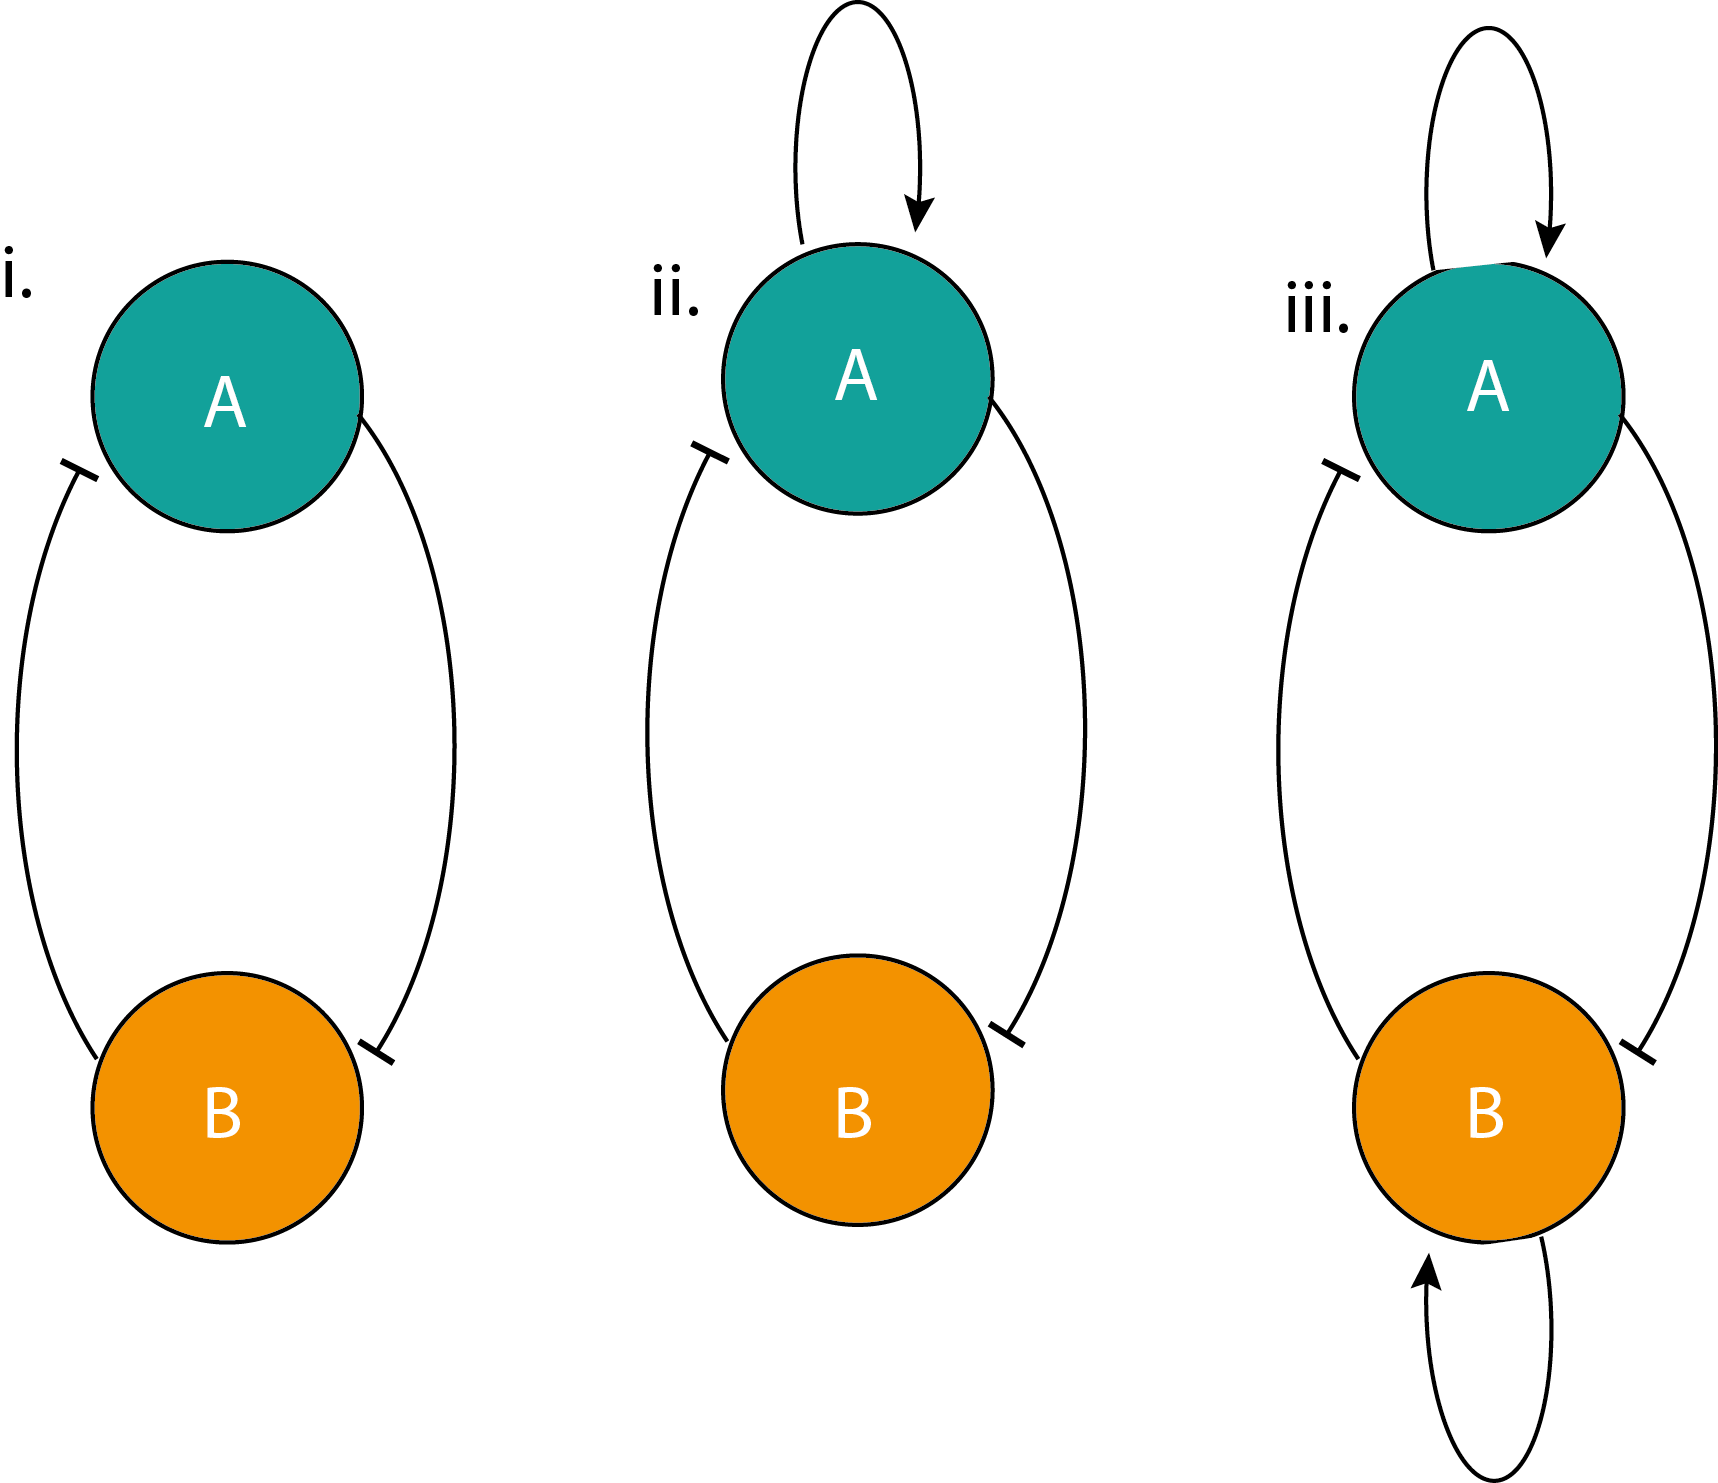
\includegraphics[scale=0.5]{chapterStabilityFinder/Lu_switches/images/lu_three_switches_sketch.png}
\caption[Lu switches]{The three Lu switches studied. (i) is the classical model with no self activation, (ii) has a single positive autoregulation and (iii) has double positive autoregulation. }
\label{fig:lu_sketch}
\end{figure}


\clearpage

\subsection{Classical model}
For the classical model, in which no self-activation is present, the system reduces to the following equations:

\begin{align}
\dot{x}=f_{x}(x,y) &= g_{x}H^{S}_{xy}(y)-k_{x}x,\label{eq:lu_cl_1}\\
\dot{y}=f_{y}(x,y) &= g_{y}H^{S}_{yx}(x)-k_{y}y\label{eq:lu_cl_2}
\end{align}
For the parameter values used in the Lu study, as shown in Table ~\ref{tab:lu_cl_bi}, the system exhibits three steady states (Figure ~\ref{fig:lu_bis_class}), of which two are stable and one is unstable. 

\begin{table}[htbp]
\centering
\caption{Lu classical model parameter values}
\label{tab:lu_cl_bi}
\begin{tabular}{cccccccccc}
gx    & gy    & kx    & ky    & nxy & nyx & xxy     & xyx     & Ixy   & Iyx \\
40&40     &0.1   & 0.1   &  3  &  3  &  200    &  200    & 0.1    &   0.1
\end{tabular}
\end{table}

\begin{figure}[htbp]
\centering
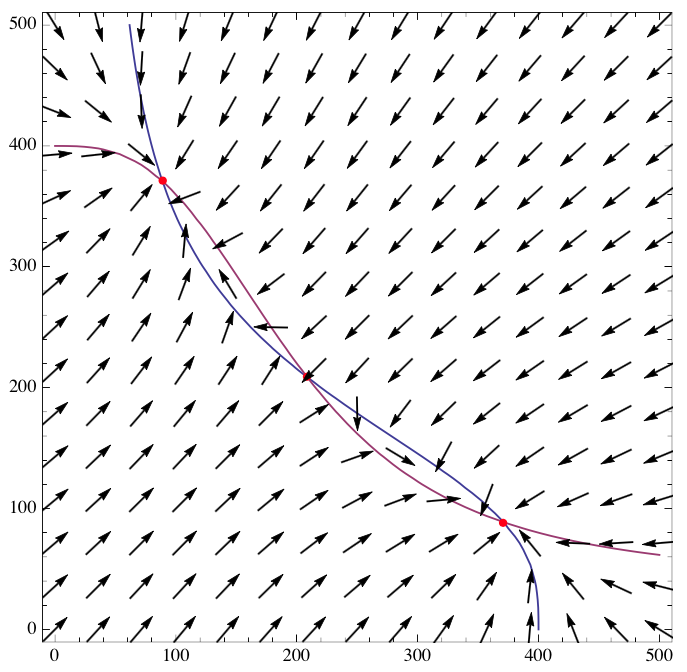
\includegraphics[scale=0.4]{chapterStabilityFinder/Lu_switches/images/mae/classical_bistable.png}
\caption[Phase portrait of the Lu classical model with no self activation]{Phase portrait of the Lu classical model with no self activation. There are two stable steady states and one unstable steady state.}
\label{fig:lu_bis_class}
\end{figure}


\clearpage

Using StabilityFinder with priors centred around the parameter values used in the original paper (Table ~\ref{tab:lu}), we can find the robustness of this bistable behaviour, as well as identify the most important parameters for bistability. 
\begin{table}[h]
\centering
\caption{Lu classical model priors}
\label{tab:lu}
\begin{tabular}{cccccccccc}
gx    & gy    & kx    & ky    & nxy & nyx & xxy     & xyx     & Ixy   & Iyx \\
35-45 & 35-45 & 0-0.2 & 0-0.2 & 2-4 & 2-4 & 150-250 & 150-250 & 0-0.2 &   0-0.2 
\end{tabular}
\end{table}

The posterior distribution of this model is shown in Figure~\ref{fig:lu_bistable}. As can be seen from the posterior, the most restrained parameters are kx and ky, the parameters responsible for the degradation of the species involved. This indicates that the rate of degradation of the species is critical for the desired dynamic to occur. 

\begin{figure}[htbp]
\centering
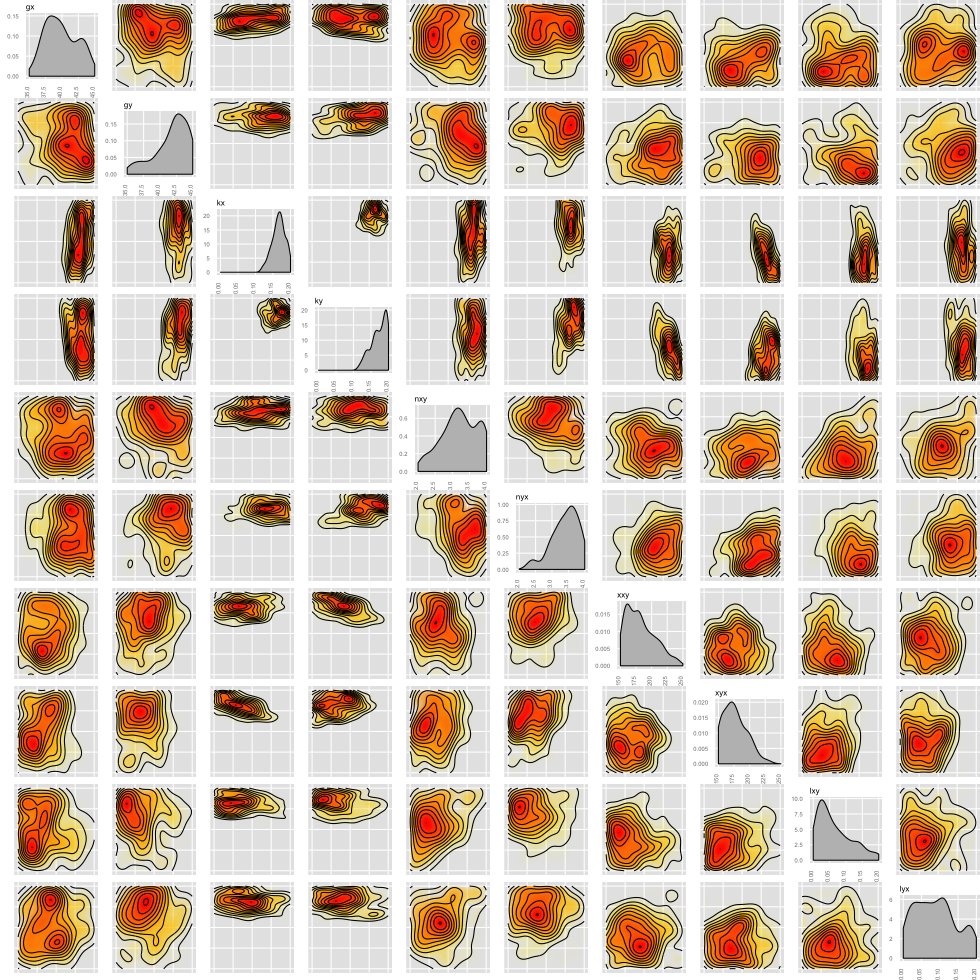
\includegraphics[scale=0.25]{chapterStabilityFinder/Lu_switches/images/classic/posterior_lu_cl.png}
\caption[The posterior distribution of the Lu classical model with no self activation]{The posterior distribution of the Lu classical model with no self activation. kx and ky are the most constrained parameters.}
\label{fig:lu_bistable}
\end{figure}

\begin{figure}[htbp]
\centering
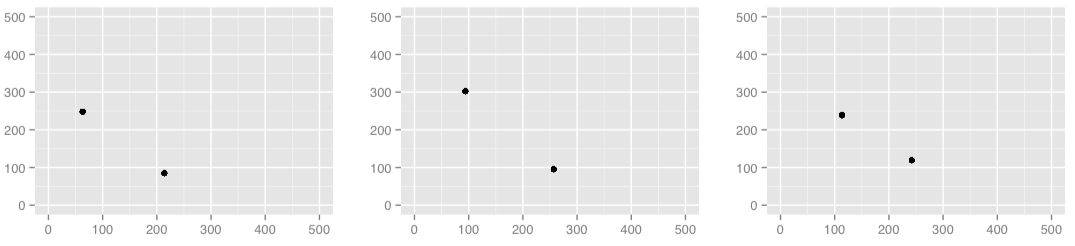
\includegraphics[scale=0.2]{chapterStabilityFinder/Lu_switches/images/classic/phase_plot.png}
\caption{A sample of the phase plots produced from the final population of the Lu classical model.}
\label{fig:lu_phase}
\end{figure}
\clearpage

\subsection{Single positive autoregulation}

If single self-activation is included, then the system is that presented in equations \ref{eq:lu_both_1} - \ref{eq:lu_hmx}. Using the priors used in Table~\ref{tab:lu_sp_pr}, the posterior distribution of for this bistable switch is that shown in Figure~\ref{fig:lu_sp_pos}. 

\begin{table}[htbp]
\centering
\caption{Lu model with single self-activation priors}
\label{tab:lu_sp_pr}
\begin{tabular}{cc}
parameter & range \\
gx & 1-2 \\
gy & 20-25 \\
kx & 50-55 \\
ky & 48-52 \\
nxy & 30-35 \\
nyx & 0.1-0.2 \\
xxy & 2-3 \\
xyx & 0.4-0.6 \\
lxy & 0.02-0.04 \\
lyx & 0.02-0.04 \\
nXX & 25-30  \\
nYY & 0.01-0.02 \\
xXX & 0.4-0.5 \\
xYY & 1-3 \\
lXX & 65-72 \\
lYY & 0.02-0.04
\end{tabular}
\end{table}


\begin{figure}[t]
\centering
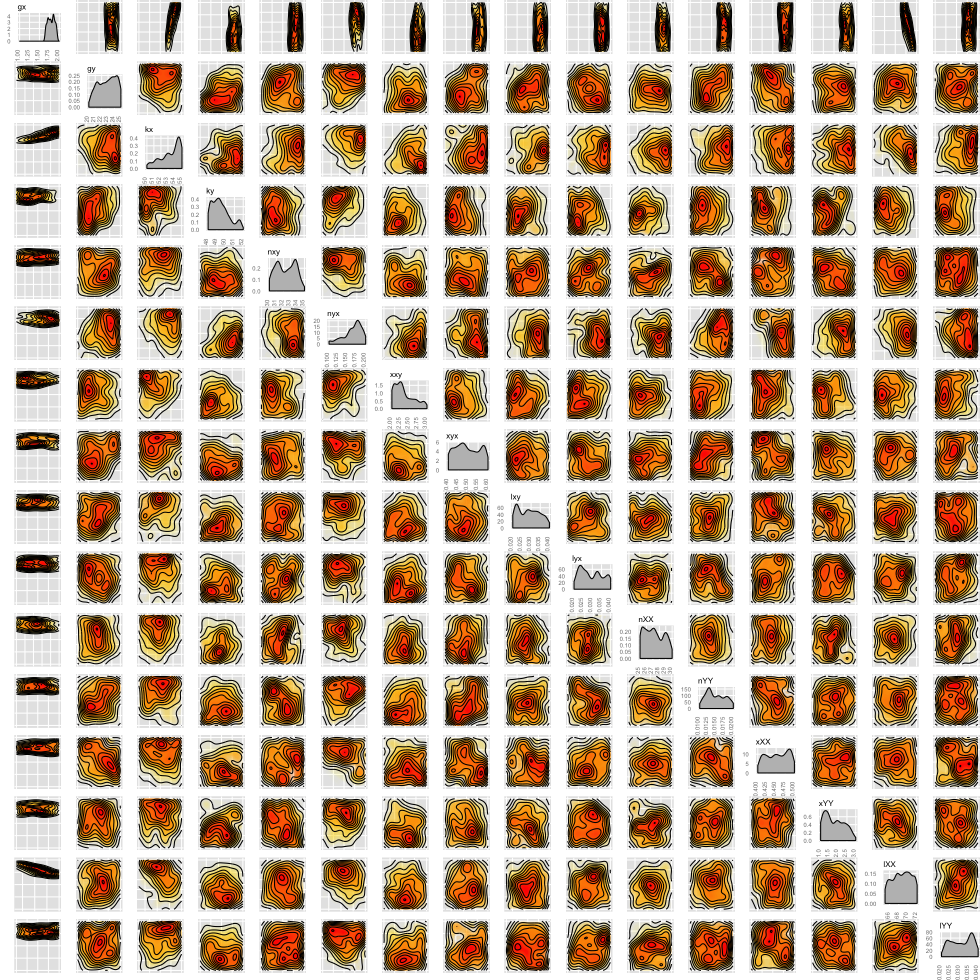
\includegraphics[scale=0.35]{chapterStabilityFinder/Lu_switches/images/single_pos/posterior_lu_sp_bis.png}
\caption[The posterior distribution of the Lu model with asymmetric self activation]{The posterior distribution of the Lu model with asymmetric self activation}
\label{fig:lu_sp_pos}
\end{figure}

\begin{figure}[t]
\centering
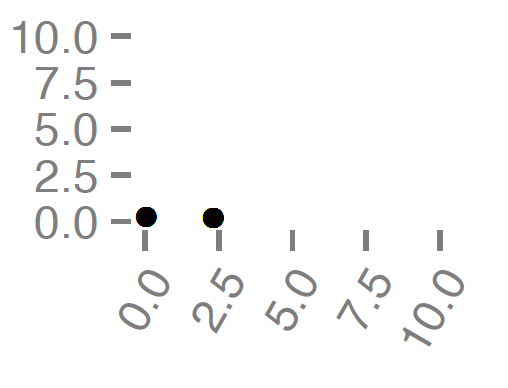
\includegraphics[scale=0.2]{chapterStabilityFinder/Lu_switches/images/single_pos/phase_plot.png}
\caption{Phase plot of asymmetric Lu toggle switch}
\label{fig:lu_sp_phase}
\end{figure}
\clearpage

\subsection{Double positive autoregulation}
If self-activation is included, then the system is that presented in equations \ref{eq:lu_both_1} - \ref{eq:lu_hmx}. When values that are presented in Table~\ref{tab:lu_dp_tri} are assigned to the parameters for the self-activating model, the system exhibits three stable and two unstable steady states as seen in Figure~\ref{fig:lu_tri_phse}. 

\begin{table}[h]
\centering
\caption{Lu model with self-activation parameter values}
\label{tab:lu_dp_tri}
\begin{tabular}{cccccccccc}
gx    & gy    & kx    & ky    & nxy & nyx & xxy     & xyx     & Ixy   & Iyx \\
4&4     &0.1   & 0.1   &  1  &  1  &  200    &  200    & 0.1    &   0.1
\end{tabular}
\end{table}

\begin{figure}[h]
\centering
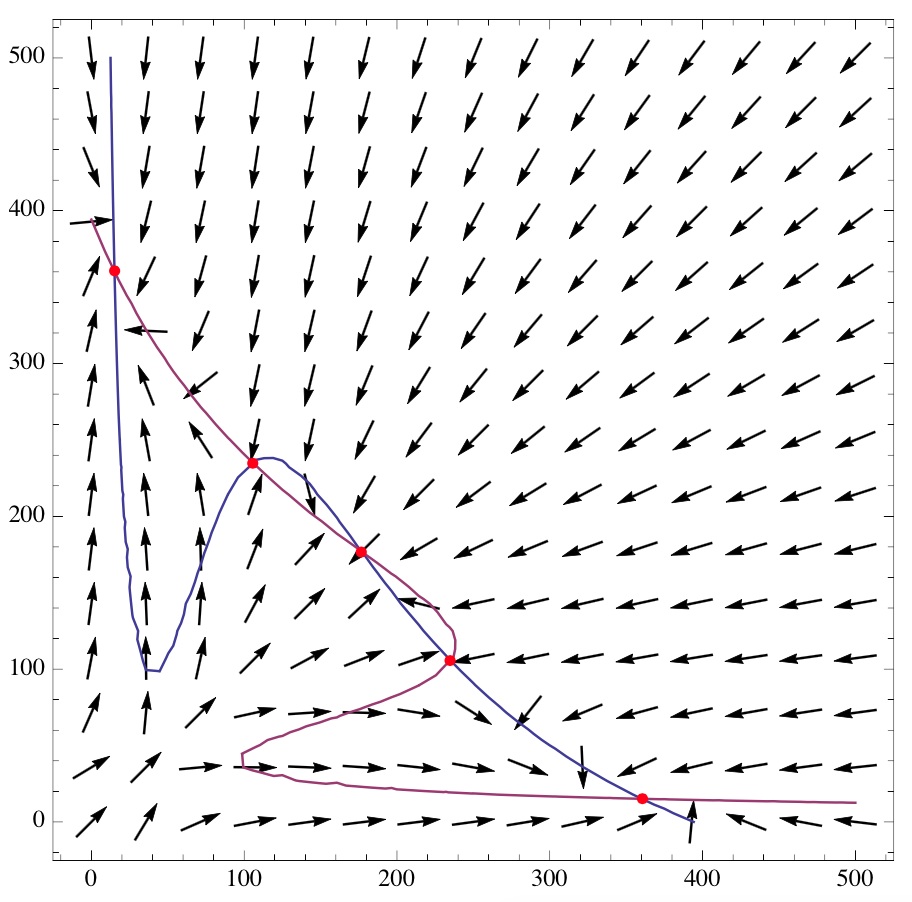
\includegraphics[scale=0.3]{chapterStabilityFinder/Lu_switches/images/mae/tristable_db.png}
\caption[Phase portrait of the Lu model including double self-activation]{Phase portrait of the Lu model including double self-activation. The model had three stable steady states and two unstable steady states.}
\label{fig:lu_tri_phse}
\end{figure}
\clearpage
Using StabilityFinder and wide priors around the original values, shown in Table~\ref{tab:lu_dp_pr}, we can explore the robustness of this behaviour, in a similar way as done for the classical model. 

\begin{table}[htbp]
\centering
\caption{Lu model with double self-activation priors}
\label{tab:lu_dp_pr}
\begin{tabular}{cc}
parameter & range \\
gx & 1-100 \\
gy & 1-100 \\
kx & 0-1 \\
ky & 0-1 \\
nxy & 0-10 \\
nyx & 0-10 \\
xxy & 100-1000 \\
xyx & 100-1000 \\
lxy & 0-1 \\
lyx & 0-0.2 \\
nXX & 0-10  \\
nYY & 0-10 \\
xXX & 50-500 \\
xYY & 50-500 \\
lXX & 1-20 \\
lYY & 1-20
\end{tabular}
\end{table}

The posterior is shown in Figure~\ref{fig:lu_tristable}. 
\begin{figure}[h]
\centering
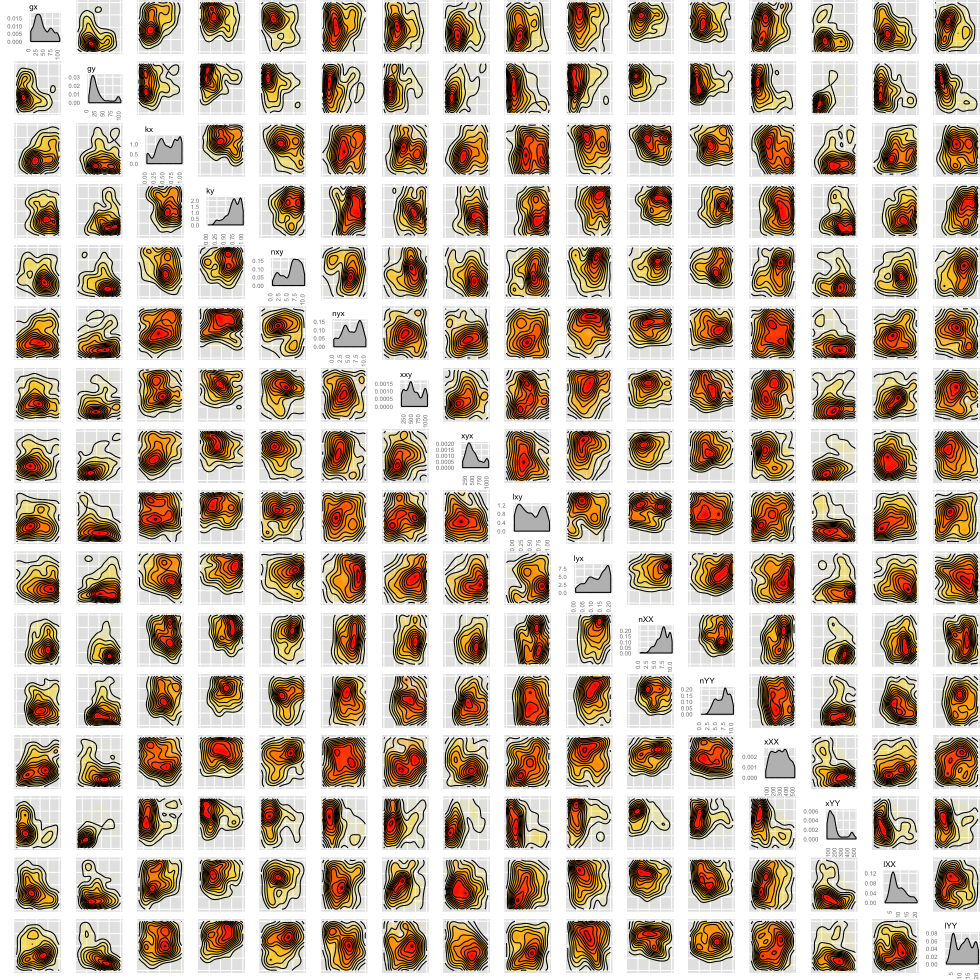
\includegraphics[scale=0.4]{chapterStabilityFinder/Lu_switches/images/double_pos/posterior_tri_wide_params.png}
\caption[The posterior distribution of the Lu model with double self activation]{The posterior distribution of the Lu model with double self activation.}
\label{fig:lu_tristable}
\end{figure}


\begin{figure}[h]
\centering
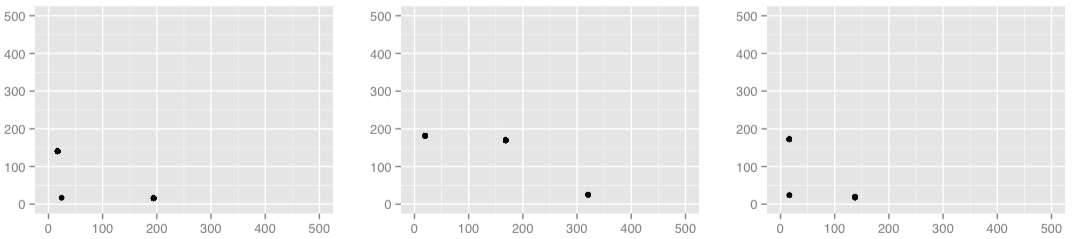
\includegraphics[scale=0.3]{chapterStabilityFinder/Lu_switches/images/double_pos/phase_plots.png}
\caption{A sample of the phase plots produced from the final population of the Lu tristable model.}
\label{fig:lu_tri_phase_pl}
\end{figure}
\clearpage
%%%%
\subsection{Extracting the design principles of a tristable switch}
Next, we went on to study the design principles that make a switch tristable vs bistable. In order to do that, first we use StabilityFinder to find the parameter space that gives rise to a bistable switch, given the same model and priors used above to find a tristable switch, as shown in Figure~\ref{fig:lu_bi_tri_cartoon}.

\begin{figure}[h]
\centering
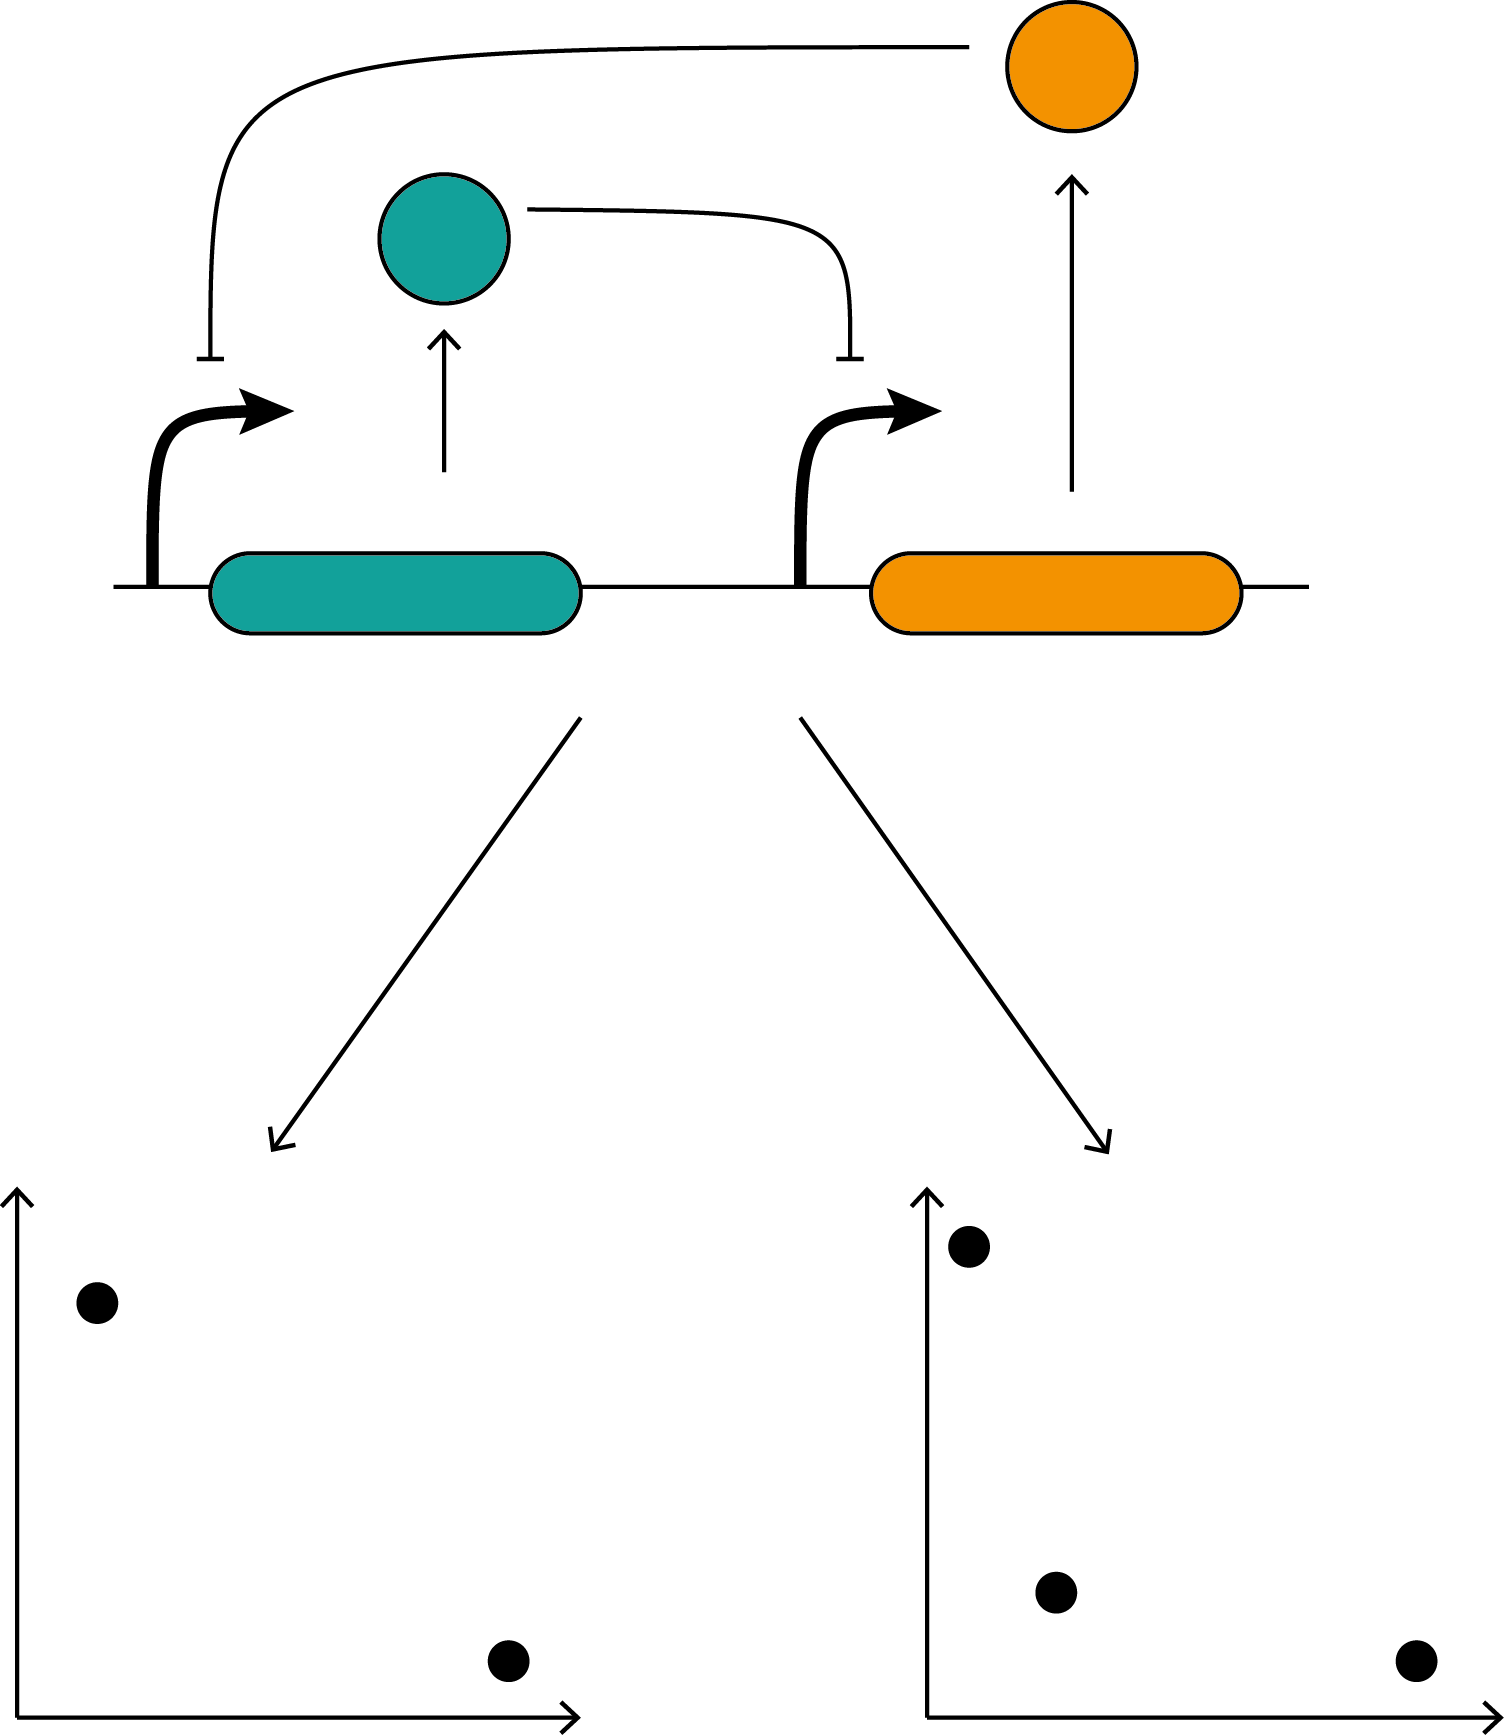
\includegraphics[scale=0.5]{chapterStabilityFinder/Lu_switches/images/double_pos/lu_bi_tri_cartoon.png}
\caption{Finding the parameter spaces that make the Lu double positive model bistable and tristable. }
\label{fig:lu_bi_tri_cartoon}
\end{figure}

By plotting the resulting posterior with that of the tristable switch shown in Figure~\ref{fig:lu_tristable} we can examine any separation of values between a bistable and a tristable switch, as shown in Figure~\ref{fig:pos_comp_lu}.

\begin{figure}[h]
\centering
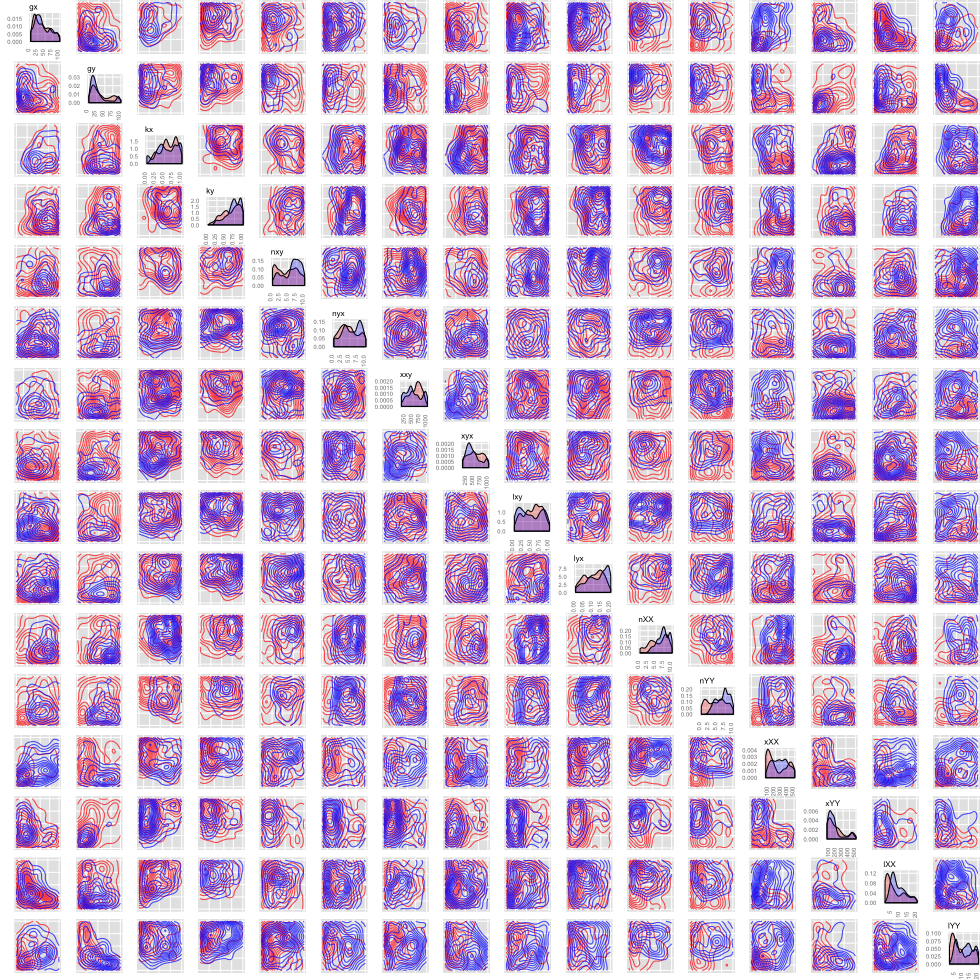
\includegraphics[scale=0.4]{chapterStabilityFinder/Lu_switches/images/double_pos/posterior_comparison_bi_tri.png}
\caption{Comparing the posteriors of the tristable Vs bistable Lu switch.}
\label{fig:pos_comp_lu}
\end{figure}
\clearpage

In order to separate the values in a more meaningful way, we implement an algorithm as outlined in Appendix. By taking samples from the posterior of a bistable switch, we keep track of the values for each parameter that are also found in the posterior of the tristable switch, and vice versa. The results are shown in Figure~\ref{fig:design_princip_lu} below:


\begin{figure}[h]
\centering
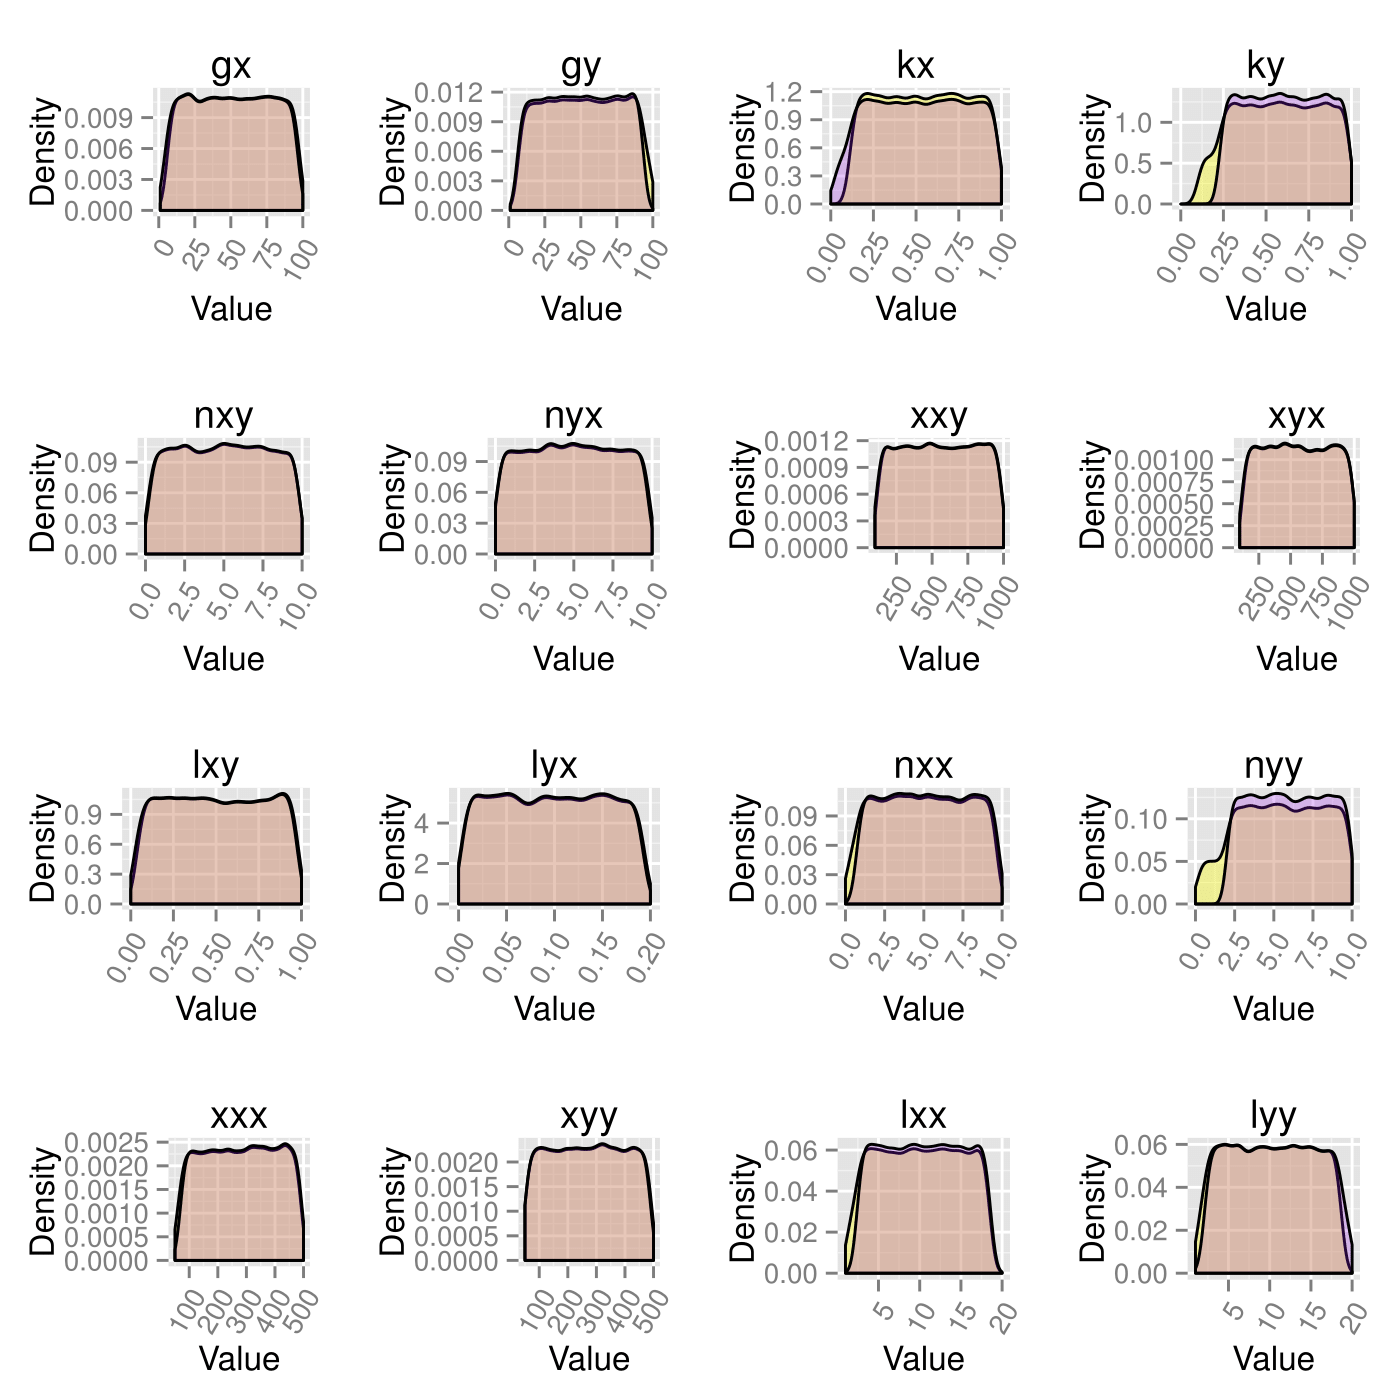
\includegraphics[scale=0.2]{chapterStabilityFinder/Lu_switches/images/double_pos/design_principles_bi_tri.png}
\caption{Design principles of the tristable Lu switch.}
\label{fig:design_princip_lu}
\end{figure}

From the results above we can conclude that there is no significant difference between a bistable and a tristable switch in parameter values. 

